\chapter{Motivación y Contexto}

\section{Introducción}

La fotónica es la ciencia que estudia la generación, detección y manipulación de la luz. 
Los principales beneficios que ofrece son \citep{Shen2019}:
% TODO: Buscar si hay una mejor referencia que ponga explícitamente estas ventajas
(i) elevado ancho de banda en comunicaciones, 
(ii) bajo consumo energético,
(iii) interconexiones ópticas independientes de la distancia.
Asimismo, existen propuestas que aprovechan estos beneficios, por ejemplo:
(i) interconexiones ópticas en centrales de datos \citep{Shen2019}, % Este paper es de la profesora Keren
(ii) redes neuronales ópticas \citep{Shen2017} e %Este paper ya es de la prof. Keren
(iii) internet de las cosas \citep{Li2021}.


%\jorge{definir fotonica es la ciencia que estudia y manipula luz... etc y es usado en aplicaciones diarias como .... dar otros ejemplos}.
%\jorge{rewrite: La fotónica es una ciencia que utilizamos diariamente, por ejemplo, mediante los cables ópticos.}
%Los principales beneficios que ofrece \jorge{son \citep{Glick2018}:} (i) elevado ancho de banda en comunicaciones, (ii) bajo consumo energético, (iii) interconexiones ópticas independientes de la distancia.
%\jorge{ mover al inicio a la, estos serían los ejemplos}.
%\jorge{rewrite:El potencial de la fotónica se logra evidenciar en aplicaciones que aprovechan estos beneficios;} por ejemplo,
%(i) interconexiones ópticas en centrales de datos \jorge{ usar un paper de Keren}\citep{Shen2019}, 
%(ii) redes neuronales ópticas \jorge{paper keren, natalie dnn with optical switches} \citep{Shen2017}, 
%(iii) internet de las cosas \jorge{cambiar de citacion} \citep{Glick2018}.

Un problema presentado en el Top500 sistemas de computación de alto desempeño (HPC, por sus siglas en Inglés) es que desde el año 2010, 
el ratio entre el ancho de banda entre nodos y el poder de procesamiento por nodo ($byte / FLOP$) ha decrecido en un factor de seis.
Es decir, se está llegando a un punto donde la capacidad para interconectar nodos está
limitando el desempeño de sistemas HPC en programas que hacen uso extensivo de transferencias de memoria.
Ante este problema, los avances en la fotónica en silicio (SiP) integrada se presenta como una de las principales alternativas de solución. 
Esta propuesta puede realizar interconexiones a distancias del orden de metros,
manteniendo un elevado ancho de banda y bajo consumo energético \citep{Shen2019, Anderson2018}.

%\jorge{ser directo: La fotónica es una de las principales alternativas de interconexión para los sistemas de comp alto desem (del ingles, High Performance Computing)}
%\jorge{remover}La importancia de estas aplicaciones en computación se evidencia aún más en la computación de alto rendimiento (HPC).
%\jorge{ Desde el 2010, el ratio entre el ancho de banda entre nodos y el poder de procesamiento por nodo ($byte / FLOP$) en sistemas HPC ha decrecido en un factor de seis. EXPLICAR simple: es necesario mantener la data en el nodo evitando transferencia, o algo similar}.
%Un problema presentado en el Top500 sistemas HPC es que desde el año 2010, el ratio entre el ancho de banda entre nodos y el poder de procesamiento por nodo ($byte / FLOP$) ha decrecido en un factor de seis.
%\jorge{remover:Así,} se está llegando a un punto donde la capacidad para interconectar nodos está limitando el desempeño de sistemas HPC en programas que hacen uso extensivo de transferencias de memoria.
%Ante este problema se han propuesto arquitecturas que aprovechan \jorge{el contexto de transmitancia es incorrecto, reescribir, usar interconexión óptica} la transmitancia óptica porque esta puede realizar interconexiones a distancias del orden de metros. 
%\jorge{remover: repeating yourself con el primer párrafo}De esta manera se logra la transferencia de grandes cantidades de información con un bajo consumo energético y manteniendo un elevado ancho de banda \citep{Shen2019, Anderson2018}.

A pesar del avance en el diseño e integración de dispositivos SiP, en términos
de cantidad de dispositivos por chip, la fotónica integrada aún se encuentra en la misma etapa de expansión que tenía la
electrónica en los años 1970s \citep{LukasChrostowski2010}.
Sin embargo, ya existen procesos de fabricación estándar en \emph{foundries}
para fabricar chips SiP, a un precio accesible, utilizando procesos CMOS
a través del \emph{process design kit} (PDK) \citep{Bogaerts2018}.
De este modo, se facilita el desarrollo de esta tecnología.


En el área de SiP integrada, la alta densidad de fabricación es un desafío
porque se requiere mantener eficiencia en el chip a nivel de sistema fotónico;
por ello, se está buscando optimizar dispositivos fundamentales que lo compongan \citep{Vuckovic2019}.
Para esto existen dos estrategias principales: (i) diseño tradicional
\citep{Hughes2016, Song2008, Huang2018} y (ii) diseño inverso \citep{Malheiros-Silveira2020, Gregory2015, Su2020}.


%SiP \jorge{ El diseño de dispositivos SiP} \jorge{ se estudia para aumentar la ciencia, el potencial mostrado es una consecuencia reescribir:} se está estudiando con el fin de mostrar el potencial de la fotónica, 
%\jorge{ reescribir: a pesar del avance en diseño e integración de SiP dispositivos, la óptica integrada aun se encuentra en la misma etapa de expansio... recordar que esto es a nivel de densidad (Cantidad de devices sip en chip} pero esta tecnología aún se encuentra en la misma etapa de expansión que tenía la electrónica en los años 1970s.
%Afortunadamente,\jorge{ cambiar por Actualmente, } ya existen \jorge{procesos de fabriación estandar en foundries CITE para integración con dispositivos CMOS a través de process design kit (PDK)}.  \emph{foundries} y procesos como el CMOS que se pueden emplear como infraestructura para la fabricación de chips SiP \citep{LukasChrostowski2010}.
%Pero, \jorge{no comenzar las oraciones con pero, puede ser sin embargo,} los chips SiP siguen siendo ineficientes \jorge{esta aseveración es categòrica y equivocada. reescribir: } por lo cual se está buscando optimizar dispositivos fundamentales que lo componen \citep{Vuckovic2019}.
%Para esto existen dos estrategias \jorge{principales}: \jorge{(i) diseño tradicional CITACIONES} y (ii) diseño inverso \jorge{citaciones}.


%\jorge{esta afirmación es categòrica y equivocada, existen sistemas con moduladores y qsfp+ desde hace años} Las aplicaciones señaladas anteriormente demuestran el potencial de la fotónica, mas estas aún no logran ponerse en práctica. 
%\jorge{ reescribir: la alta densidad de fabricación es un desafío porque se requiere mantener eficiencia en el chipo a nivel de sistema fotónico}
%Para que cada una de ellas funcione se necesita fabricar chips de fotónica integrada con una elevada eficiencia y densidad.
%\jorge{ necesita contexto de eficiencia, a que te refieres?}
%Pero los diseños actuales aún son muy ineficientes por lo cual sigue conviniendo utilizar dispositivos electrónicos \citep{Glick2018, Vuckovic2019}. 
%Ante esta dificultad, la fotónica en silicio (SiP) se presenta como un buen candidato para fabricar estos chips.
%La idea se refuerza por la adaptación de procesos de semiconductor complementario de óxido metálico (CMOS) para fabricar dispositivos SiP.
%Esto es un gran beneficio porque los procesos CMOS son una tecnología bien establecida y con precios accesibles \citep{Glick2018, Shen2019, LukasChrostowski2010}.


\begin{figure}[ht]
  \centering
  % 1° row
  % Traditional bend
  \subfigure[\emph{Bend} con diseño
  tradicional.]{
\includegraphics[width=0.4\textwidth]{image/introduction/traditional-bend.png}}
  \hfill
  % Inverse design bend
  \subfigure[\emph{Bend} obtenido con diseño inverso. Extraído de
  \citep{Su2020}.]{
    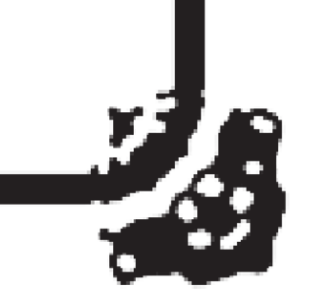
\includegraphics[width=0.4\textwidth]{image/introduction/inverse-design-bend.png}
  }

  % 2° row
  % Traditional splitter
  \subfigure[WDM con diseño tradicional.]{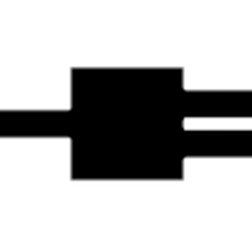
\includegraphics[width=0.4\textwidth]{image/introduction/traditional-splitter.png}}
  \hfill
  % Inverse design splitter
  \subfigure[WDM obtenido con diseño inverso. Extraído de \citep{Su2020}.]{
    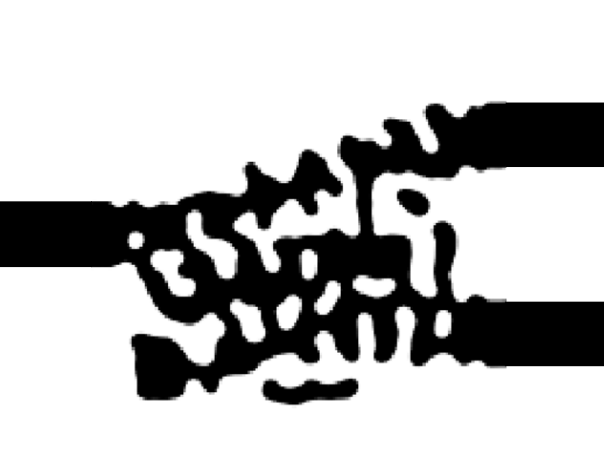
\includegraphics[width=0.4\textwidth]{image/introduction/inverse-design-splitter.png}
  }

  \caption{Diseños tradicionales y obtenidos a partir de diseño inverso de un
  \emph{bend} y un WDM.}
  \label{fig:devices}

\end{figure}


La figura \ref{fig:devices} presenta una comparación de los dos tipos de diseño
(tradicional e inverso) en dos dispositivos: (i) \emph{bend-90°} y (ii)
\emph{wavelength demultiplexer} de dos canales (WDM).
Como se observa en la figura \ref{fig:devices}, en el diseño tradicional (izquierda) se define el dispositivo con geometrías simples que permiten obtener funciones analíticas de sus propiedades físicas \citep{Hughes2016, Song2008}. 
Esto se realiza para poder optimizar la función obtenida a partir de los parámetros que la definan. 
Dicha optimización se suele ejecutar haciendo un barrido de los parámetros, con algoritmos genéticos o usando \emph{particle swarm optimization}. 
Esta técnica es un enfoque simple, pero que ha obtenido buenos resultados
\citep{Su2020}. 


Sin embargo, existen tres grandes inconvenientes con el diseño tradicional. 
Primero, solamente se explora una pequeña fracción de todos los posibles diseños.
Segundo, por lo general no es conocido el límite de rendimiento del dispositivo
\citep{Molesky2018}.
Tercero, al trabajar en la escala de nanómetros, existen casos como el
\emph{bend-90°} y WDM que presentan un bajo rendimiento \citep{Su2020}.

%\jorge{La Figura XX presenta una comparación de los dos tipos de diseño (Tradicional e inverso) en dos devices (bend y MUX)}
%En el diseño tradicional se define el dispositivo con geometrías simples que permiten obtener funciones analíticas de sus propiedades físicas \citep{Hughes2016, Song2008}. 
%Esto se realiza para poder optimizar la función obtenida a partir de los parámetros que la definan. 
%Dicha optimización se suele ejecutar haciendo un barrido de los parámetros,
%con algoritmos genéticos o usando \emph{particle swarm optimization}.%Es un enfoque simple, pero que ha obtenido buenos resultados. 
%\jorge{escribir algo como: se observa en la Fig. XX (izquierda) geometrías regulares o de un patrón casi uniforme para ambos devices...}
%Sin embargo, existen tres grandes inconvenientes con este planteamiento. 
%Primero, \jorge{ solamente se explora} solo estamos explorando una pequeña fracción de todos los posibles diseños.
%Segundo, por lo general no es conocido el límite de rendimiento del dispositivo.
%Tercero, al trabajar en la escala de nanómetros, existen casos como el \emph{bend} y WDM que presentan un bajo rendimiento con diseños tradicionales \citep{Molesky2018, Su2020}.


Por el otro lado, en el diseño inverso, mostrado en la figura \ref{fig:devices}
(derecha), las geometrías resultantes no están limitadas a diseños intuitivos o regulares.
Esta técnica busca hacer una mayor exploración de todos los posibles diseños.
Para ello, se define geometrías arbitrarias y se usa simulaciones
computacionales para determinar las propiedades físicas del dispositivo,
propiedades que son usadas para formular una función objetivo.
Finalmente, se aplican algoritmos de optimización para encontrar valores
óptimos de esta función \citep{Molesky2018, Su2020}.
Para una descripción detallada de los distintos algoritmos de optimización
comúnmente empleados, por favor revisar \cite{Schneider2019, Elsawy2020, Campbell2019}.

%En el diseño inverso, figura \ref{fig:devices} (derecha), se busca hacer una mayor exploración de todos los posibles diseños. 
%\jorge{La Figura xx (derecha) muestra que el diseño inverso las geometrías resultantes no están limitadas a diseños intuitivos o regulares}
%\jorge{remover:Para ello, ya no nos limitamos a solo usar diseños intuitivos, ver figura \ref{fig:devices}}. 
%\jorge{ Se definen geometrias arbitrarias generadas a partir de simulaciones computaciones (el diseño tradicional no usa simulación o cálculo? tener cuidado con esto reescribir...}Ahora, definimos geometrías arbitrarias y usamos simulaciones computacionales para determinar las propiedades físicas del dispositivo \citep{Molesky2018, Su2020}. 

El diseño inverso ha logrado conseguir mejores resultados que los obtenidos por el
diseño tradicional por lo que ha ganado interés en el área de fotónica durante
los últimos 20 años \citep{Su2018, Molesky2018, Campbell2019}. 
% volver a revisar Campbell2019
Sin embargo, existen cuatro grandes desafíos con este planteamiento:
(i) el espacio de búsqueda es exponencial \citep{Vuckovic2019}, 
(ii) las simulaciones computacionales son costosas en términos de tiempo y memoria \citep{Kudyshev2020}, 
(iii) el espacio de búsqueda es no convexo \citep{Su2018} y
(iv) no todos los diseños son fabricables \citep{Su2020}.


%Este enfoque ha logrado conseguir mejores resultados que los obtenidos por el diseño tradicional \citep{Su2018, Molesky2018} \jorge{juntar con: por lo que ha ganado spotlight en fotónica durante los} últimos 20 años \citep{Molesky2018} \jorge{se necesitan mas papers CITE}.
%Sin embargo, este planteamiento viene acompañado de nuevos desafíos.



%\jorge{ Se deben incorporar restricciones ... CITE} \jorge{reescribir: están dándose razones de dificultad o desafíos del diseño inverso, cada uno debe tener citaciones} \cite{Su2018, Piggott2017} se incorporan restricciones de fabricación para obtener dispositivos que al fabricarse mantengan un buen rendimiento. 
%No obstante, la búsqueda de estos diseños suele realizarse aplicando algoritmos cuya selección y configuración es mayormente debido a un tedioso proceso de prueba y error \jorge{ CITE}.
%Otros trabajos como los de \cite{Schneider2019, Elsawy2020, Gregory2015} comparan distintos algoritmos de optimización en el diseño inverso de dispositivos fotónicos. \jorge{esta parrafo anterior debe ser reescrito, parece una revisión de trabajos, necesitamos resaltar los desafíon principales, y que sobre todo si hay viabilidad de superarlos}

Y aún cuando una cantidad considerable de investigaciones estudian dispositivos
SiP \citep{Su2018, Malheiros-Silveira2020}, sigue siendo necesario estudiar dispositivos SiP
fundamentales para conseguir chips de SiP integrada densos y eficientes.
Los avances en esta área benefiarán indirectamente al desarrollo de Ciencia de
la Computación con mejoras en el \emph{hardware} utilizado para ejecutar
eficientemente, por
ejemplo, programas de inteligencia artificial o de computación de alto
desempeño.

De este modo, el presente trabajo se centra en estudiar dos dispositivos SiP
fundamentales:
(i) \emph{bend-90°} y (ii) \emph{wavelength demultiplexer} de dos canales.
De aquí en adelante nos referiremos a estos simplemente como \emph{bend} y WDM.
Por lo tanto, el objetivo de esta tesis es aplicar el conocimiento en computación para
encontrar diseños de estos dispositivos con eficiencias mayores al 90\%
y resilientes a errores de fabricación, trabajando en la escala de nanómetros.
Con el fin de solucionar este problema se empleará diseño inverso para encontrar geometrías con las eficiencias deseadas, 
para ello se realizará simulaciones computacionales con cinco algoritmos de optimización populares. 
De este modo, se espera obtener diseños cuyas simulaciones presenten las características señaladas y 
que, potencialmente, muestren propiedades similares al fabricarse.


%\jorge{WDM es wavelength division multiplexing, el término comun en literatura es WDM mux/demus corregir}, \jorge{remover:respectivamente}.


%Aún \jorge{remover: cuando una cantidad considerable} de investigaciones están usando el diseño inverso para optimizar dispositivos fotónicos, el \emph{bend} y WDM, dispositivos fundamentales para los circuitos fotónicos, aún no logran aplicación comercial \citep{Molesky2018}. \jorge{ A pesar qaue múltiples trabajos ...}
%Además, existe una carencia de estudios con un enfoque computacional que intenten abordar el problema. \jorge{citacion}
%Asi, \jorge{remover así,  directo} el objetivo de esta tesis es aplicar el conocimiento en computación para optimizar estos dispositivos y conseguir diseños que al fabricarse muestren un desempeño elevado.



%\jorge{reescribir y aprovechar para introducir tu contexto: diversos o múltiples trabajos son orientados al diseño de geometrías de dispositivos fotónicos, si haces esta afirmación debes citar realmente múltiples trabajos CITE}
%Por estos motivos, una cantidad considerable de investigaciones estudian dispositivos SiP \citep{Molesky2018}.
%El presente trabajo se centrará en dos de ellos: \jorge{(i)} \emph{bend-90°} y \jorge{(ii)}\emph{wavelength demultiplexer} de dos canales.
%\jorge{footnote:} De aquí en adelante nos referiremos a estos simplemente como \emph{bend} y WDM \jorge{WDM es wavelength division multiplexing, el término comun en literatura es WDM mux/demus corregir}, \jorge{remover:respectivamente}.

El presente documento está organizado de la siguiente manera:

El capítulo 1 brinda una introducción al tema de investigación, describe el problema a detalle, justifica la relevancia de resolverlo, define los objetivos y señala los aportes del trabajo.

El capítulo 2 desarrolla conceptos fundamentales en fotónica necesarios para entender el resto del documento.

%El capítulo 2 desarrolla conceptos fundamentales en fotónica necesarios para entender el resto del documento. \jorge{listar cuales}

El capítulo 3 presenta una revisión del estado del arte en diseño inverso para
optimizar un \emph{bend} y WDM.

%El capítulo 3 presenta una revisión del estado del arte y discute sus principales características. \jorge{ el estado del arte en que? en geometrias? todas? especificar}

El capítulo 4 desbribe la metodología usada en la investigación.

%El capítulo 4 desbrine la metodología usada en la investigación. \jorge{presenta nuestra propuesta de ... especificar}

Por último, el capítulo 5 muestra los resultados obtenidos con los distintos casos de estudio. 

%El capítulo 5 muestra los resultados \jorge{remover}preliminares obtenidos con los experimentos.\jorge{presenta nuestros casos de estudio y el setup experimental, así como los resultados obtenidos}.

%La fotónica está atrayendo el interés de la industria debido a su potencial en términos de escalabilidad y los beneficios de costo-eficiencia \jorge{CITE, CITE, CITE}. 
%\jorge{Existen tres razones principales. remover:}Este potencial es evidente, por ejemplo, con los siguientes tres puntos. 
%Primero, si se quiere mantener la tendencia que cada 10 años se mejore en un factor de 1000 el rendimiento de los sistemas electrónicos, entonces parece ser indispensable la convergencia de estos con sistemas fotónicos \jorge{ reescribir: por que? no está claro, no hay una razón real...} \citep{Glick2018}. 
%Segundo, \jorge{reescribir, al ser el dinero la justificación necesitamos valores, existe un infográfico de un instituto en francia lo buscaré tambien.. } existe una inversión billonaria en la fabricación de transistores cuyos procesos se están adaptando para fabricar chips de fotónica integrada \citep{LukasChrostowski2010}.
%Tercero, hay prometedoras aplicaciones en \jorge{necesitas papers de la aplicación, no papers que citen otros trabajos, busca en nature} (i) interconexiones ópticas \citep{Shen2019}, (ii) redes neuronales ópticas \citep{Shen2017}e, (iii) internet de las cosas \citep{Glick2018}.
 
%SiP \jorge{ El diseño de dispositivos SiP} \jorge{ se estudia para aumentar la ciencia, el potencial mostrado es una consecuencia reescribir:} se está estudiando con el fin de mostrar el potencial de la fotónica, \jorge{ reescribir: a pesar del avance en diseño e integración de SiP dispositivos, la óptica integrada aun se encuentra en la misma etapa de expansio... recordar que esto es a nivel de densidad (Cantidad de devices sip en chip} pero esta tecnología aún se encuentra en la misma etapa de expansión que tenía la electrónica en los años 1970s.
%Afortunadamente,\jorge{ cambiar por Actualmente, } ya existen \jorge{procesos de fabriación estandar en foundries CITE para integración con dispositivos CMOS a través de process design kit (PDK)}.  \emph{foundries} y procesos como el CMOS que se pueden emplear como infraestructura para la fabricación de chips SiP \citep{LukasChrostowski2010}.
%Pero, \jorge{no comenzar las oraciones con pero, puede ser sin embargo,} los chips SiP siguen siendo ineficientes \jorge{esta aseveración es categòrica y equivocada. reescribir: } por lo cual se está buscando optimizar dispositivos fundamentales que lo componen \citep{Vuckovic2019}.
%Para esto existen dos estrategias \jorge{principales}: \jorge{(i) diseño tradicional CITACIONES} y (ii) diseño inverso \jorge{citaciones}.

%\jorge{La Figura XX presenta una comparación de los dos tipos de diseño (Tradicional e inverso) en dos devices (bend y MUX)}
%En el diseño tradicional se define el dispositivo con geometrías simples que permiten obtener funciones analíticas de sus propiedades físicas \citep{Hughes2016, Song2008}. 
%Esto se realiza para poder optimizar la función obtenida a partir de los parámetros que la definan. 
%Dicha optimización se suele ejecutar haciendo un barrido de los parámetros, con algoritmos genéticos o usando \emph{particle swarm optimization}. 
%Es un enfoque simple, pero que ha obtenido buenos resultados. \jorge{escribir algo como: se observa en la Fig. XX (izquierda) geometrías regulares o de un patrón casi uniforme para ambos devices...}
%Sin embargo, existen tres grandes inconvenientes con este planteamiento. 
%Primero, \jorge{ solamente se explora} solo estamos explorando una pequeña fracción de todos los posibles diseños.
%Segundo, por lo general no es conocido el límite de rendimiento del dispositivo.
%Tercero, al trabajar en la escala de nanómetros, existen casos como el \emph{bend} y WDM que presentan un bajo rendimiento con diseños tradicionales \citep{Molesky2018, Su2020}.


%En el diseño inverso se busca hacer una mayor exploración de todos los posibles diseños. 
%\jorge{La Figura xx (derecha) muestra que el diseño inverso las geometrías resultantes no están limitadas a diseños intuitivos o regulares}
%\jorge{remover:Para ello, ya no nos limitamos a solo usar diseños intuitivos, ver figura \ref{fig:devices}}. 
%\jorge{ Se definen geometrias arbitrarias generadas a partir de simulaciones computaciones (el diseño tradicional no usa simulación o cálculo? tener cuidado con esto reescribir...}Ahora, definimos geometrías arbitrarias y usamos simulaciones computacionales para determinar las propiedades físicas del dispositivo \citep{Molesky2018, Su2020}. 


%Este enfoque ha logrado conseguir mejores resultados que los obtenidos por el diseño tradicional \citep{Su2018, Molesky2018} \jorge{juntar con: por lo que ha ganado spotlight en fotónica durante los} últimos 20 años \citep{Molesky2018} \jorge{se necesitan mas papers CITE}.
%Sin embargo, este planteamiento viene acompañado de nuevos desafíos.

%El diseño inverso ha recibido mucha atención en fotónica durante los últimos 20 años \citep{Molesky2018}. 
%Los autores en \cite{Su2020} muestran estrategias para optimizar un \emph{bend} y \emph{WDM}.
%\jorge{ Se deben incorporar restricciones ... CITE} \jorge{reescribir: están dándose razones de dificultad o desafíos del diseño inverso, cada uno debe tener citaciones} \cite{Su2018, Piggott2017} se incorporan restricciones de fabricación para obtener dispositivos que al fabricarse mantengan un buen rendimiento. 
%No obstante, la búsqueda de estos diseños suele realizarse aplicando algoritmos cuya selección y configuración es mayormente debido a un tedioso proceso de prueba y error \jorge{ CITE}.
%Otros trabajos como los de \cite{Schneider2019, Elsawy2020, Gregory2015} comparan distintos algoritmos de optimización en el diseño inverso de dispositivos fotónicos. \jorge{esta parrafo anterior debe ser reescrito, parece una revisión de trabajos, necesitamos resaltar los desafíon principales, y que sobre todo si hay viabilidad de superarlos}


%Aún \jorge{remover: cuando una cantidad considerable} de investigaciones están usando el diseño inverso para optimizar dispositivos fotónicos, el \emph{bend} y WDM, dispositivos fundamentales para los circuitos fotónicos, aún no logran aplicación comercial \citep{Molesky2018}. \jorge{ A pesar qaue múltiples trabajos ...}
%Además, existe una carencia de estudios con un enfoque computacional que intenten abordar el problema. \jorge{citacion}
%Asi, \jorge{remover así,  directo} el objetivo de esta tesis es aplicar el conocimiento en computación para optimizar estos dispositivos y conseguir diseños que al fabricarse muestren un desempeño elevado.

\section{Descripción del Problema}


Para poder describir el funcionamiento de un dispositivo se calcula la distribución del campo eléctrico, para ello se resuelven las ecuaciones
de Maxwell \citep{Schneider2019}. 
Una forma de encontrar la solución a estas ecuaciones en cualquier geometría es utilizando un método numérico llamado diferencias finitas en el dominio de frecuencias (FDFD) \citep{Su2020}.
Con este planteamiento se selecciona una región rectangular a optimizar y se la divide  en $n \times m$  píxeles como si fuera una imagen, ver Figura \ref{fig:bend-discretization}. 
Luego, cada píxel se rellena con dos posibles materiales: óxido de silicio ($SiO_2$) o silicio ($Si$) \citep{Molesky2018}.

\begin{figure}[ht]
  \centering
  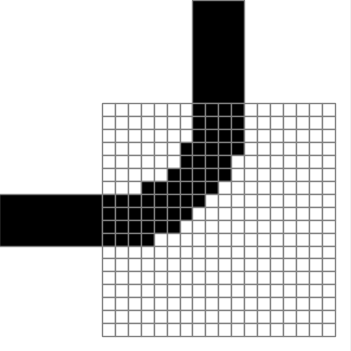
\includegraphics[scale=0.6]{image/introduction/bend-discretization.png}
  \caption{\emph{Bend} con una región de diseño discretizada en $18 \times 18$
  píxeles. Cada píxel negro representa la presencia de $Si$ y cada píxel blanco
  de $SiO_2$.}
  \label{fig:bend-discretization}
\end{figure}

El diseño inverso comienza definiendo los requerimientos del dispositivo para luego tratar de buscar entre los $2^{n \times m}$ posibles diseños algún candidato que se adapte a lo que se busca \citep{Su2020, Molesky2018}.
Como prueba de concepto, trabajos como el de \cite{Malheiros-Silveira2020} parametrizaron $2^{10 \times 10}$ posibles geometrías.
Así, se presentan algunas dificultades con esta estrategia:

\begin{enumerate}
  \item No es viable evaluar todos los posibles diseños por haber un número excesivamente elevado de ellos \citep{Vuckovic2019}.
  \item Las simulaciones computacionales son muy costosas en términos de memoria y tiempo \citep{Kudyshev2020}.
  \item El espacio de búsqueda es no convexo \citep{Su2018}.
  \item No todos los diseños son fabricables por limitaciones físicas \citep{Su2020}.
  \item Cada dispositivo es una clase distinta de problema, es decir, no necesariamente funcionará la misma estrategia para cada dispositivo \citep{Molesky2018}.
\end{enumerate}

Además, la fabricación viene con otros desafíos, principalmente:

\begin{enumerate}
  \item Errores de precisión \citep{Piggott2017}.
  \item Sensibilidad ante cambios de temperatura \citep{Vuckovic2019}.
\end{enumerate}

Considerando las anteriores dificultades, el problema es usar diseño inverso y encontrar geometrías que muestren buen desempeño en simulaciones computacionales y que puedan asegurar mantener un óptimo funcionamiento al ser fabricados. 
Este problema se estudiará para dos dispositivos nanofotónicos (i) \emph{bend} y (ii) WDM.

\section{Justificación}

El \emph{bend} y WDM son dispositivos SiP fundamentales que tienen aplicación
directa, por ejemplo, en sistemas HPC \citep{Shen2017}.
Así, las mejoras de estos ayudará indirectamente al desarrollo de Ciencia
de la Computación brindando, potencialmente, un mejor \emph{hardware} para programas de
inteligencia artificial, HPC, entre otros.
Por otro lado, desde el punto de vista computacional, este problema es interesante porque ya hay estrategias computacionales conocidas para resolverlo, desde algoritmos evolutivos \citep{Hansen2016} hasta redes neuronales \citep{Goodfellow2015} y \emph{depth learning} \citep{Malkiel2018}. 
Además, debido al alto costo computacional de las simulaciones \citep{Schneider2019}, el trabajo requiere de computación de alto desempeño.
Así, es probable que se pueda obtener buenos resultados en la investigación aplicando el conocimiento ya existente en computación. 

\section{Objetivos}

\begin{itemize}

  \item Diseñar un \emph{bend} y WDM con eficiencias mayores al 90\% y resiliente a errores de fabricación.

  \begin{itemize}

    \item Seleccionar una estrategia de parametrización que asegure facilidad de fabricación.

    \item Definir una función objetivo que encapsule las propiedades buscadas en cada dispositivo.

    \item Encontrar geometrías con valores óptimos de la función objetivo en simulaciones computacionales.

    \item Encontrar geometrías resilientes a posibles errores de fabricación de dilatación o contracción.

  \end{itemize}

  \item Comparar el desempeño y la convergencia de cinco algoritmos de optimización populares usados para optimizar dispositivos nanofotónicos.

  \begin{itemize}

    \item Implementar el proceso de optimización de los dispositivos asegurando aprovechar los
      recursos CPU de un \emph{cluster}.

    \item Implementar el proceso de optimización de los dispositivos asegurando aprovechar los
      recursos GPU de un \emph{cluster}.

  \end{itemize}

\end{itemize}



%\section{Aportes}

%Este trabajo busca brindar una comparativa de las técnicas de optimización más relevantes que se aplican para optimizar un \emph{bend} y un WDM cuando estos son parametrizados con un elevado número de variables.

%\joruge{por ahora mantener, luego alinear al paper de JLT}
